\chapter{Evaluation}
In this chapter, we introduce the provided datasets we evaluate the models on.
We then set hypotheses about the assumed performances of the chosen models on
our datasets. Next, we describe our process of training. We briefly mention the
technologies we have used and how we have chosen our models' parameters.
Finally, we present our achieved results and discuss them.

\section{Datasets}
We are provided with three datasets by the company SANEZOO. Unfortunately, two
of the datasets cannot be published as they are protected under a
confidentiality agreement. However, we provide sufficient characteristics of the
datasets. We summarize the basic information of the datasets in Table
\ref{tab:datasets}. Detailed description is provided below the table.
\todo{Doplnit chybejici udaje.}

\begin{table}[h]
	\centering
	\begin{tabular}{|l|l|l|l|l|}
		\hline
		\bld{Type}       & \bld{Difficulty} & \bld{Size}             & \bld{Classes}          & \bld{Publishable} \\ \hline
		Candies          & Easy             & 150                    & 1                      & Yes               \\
		Metal parts      & Medium           & 5790                   & 7                      & No                \\
		Medical supplies & Hard             & \textit{bude doplneno} & \textit{bude doplneno} & No                \\ \hline
	\end{tabular}
	\caption{Datasets summary.}
	\label{tab:datasets}
\end{table}


\begin{figure}[H]

	\begin{subfigure}[c]{0.5\textwidth}
		\centering
		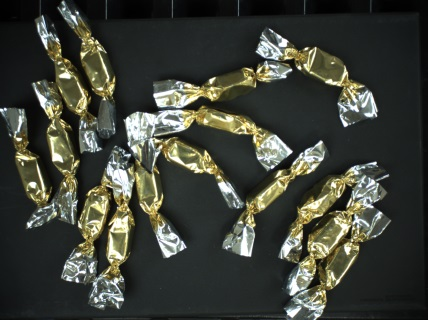
\includegraphics[width=0.9\linewidth]{Sources/Figures/sparse.jpg}
		\caption{Sparse example}

	\end{subfigure}
	\begin{subfigure}[c]{0.5\textwidth}
		\centering
		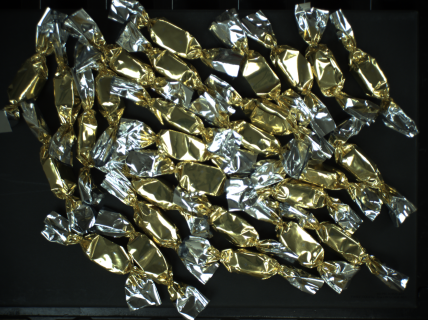
\includegraphics[width=0.9\linewidth]{Sources/Figures/dense.png}
		\caption{Dense example}

	\end{subfigure}

	\caption{Examples of candies dataset.}
	\label{fig:candies}
\end{figure}

\bld{Candies dataset.} Only the first dataset is publishable; thus, we provide a
visual example image in Figure \ref{fig:candies}. The images consist only of a
single class -- a golden candy. The density of objects (how densely they cover
the image) varies through the dataset (see Figure \ref{fig:candies}). Object
occlusions can occur in dense images; therefore, the dataset is not trivial.
However, compared to our other datasets, it is still a simpler dataset as it
strictly contains only a single class without foreign objects. Therefore, we
assign an easy difficulty to this dataset.


\bld{Metal parts dataset.} The second dataset consists of images with small
metal parts (such as shafts, rings, casings). See Figure \ref{fig:parts} for
rough illustration. The objects are placed in a plastic bin. There is always
only one class of objects on a single image. The images are taken from a
top-down perspective, similarly as in Figure \ref{fig:candies}. However, they
are taken from various angles. The density of objects also differ through the
dataset as in the first dataset (you can imagine a pile of metal parts).

\begin{figure}[ht]
	\centering
	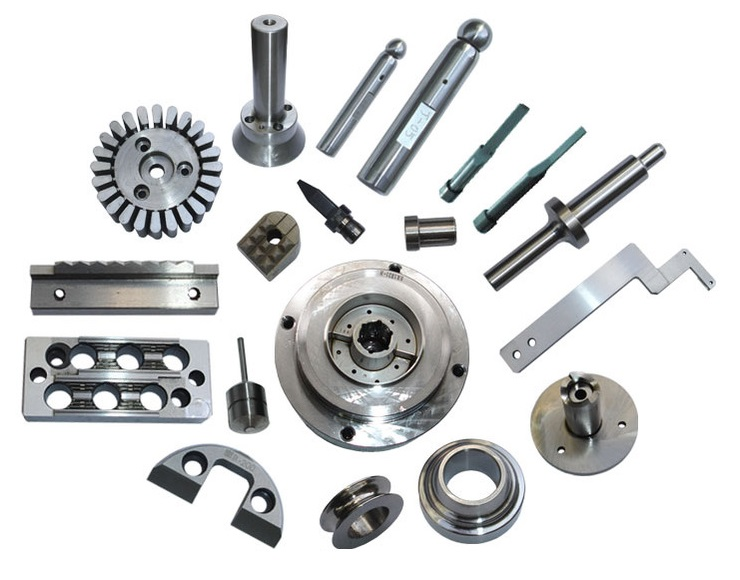
\includegraphics[height=0.35\linewidth]{Sources/Figures/metal_parts.jpg}
	\caption{An illustration of classes from metal parts dataset. Taken from
		\cite{parts}.}
	\label{fig:parts}
\end{figure}

\bld{Medical supplies dataset} The last set is made up of sequences of images
taken from an assembly line's top view. The images capture a manual assembly of
packages that are consisted of medical items (such as bandages, plastic cups, or
surgery tools). We assign a hard difficulty to this dataset because of the
non-static environment. To be more specific, the packages are in motion in some
images; therefore, the objects are slightly blurred. Moreover, occlusion of
objects occurs in the image very often since the operator does the packing
manually, and the objects are stacked on top of each other. Some objects are
tough to distinguish if they are next to each other (imagine a pile of cotton
balls). The images are taken from above the operator similarly as in the first
dataset.

\section{Hypotheses}
Let us recapitulate the models we evaluate:
\begin{itemize}
	\item Faster R-CNN with ResNet-50 backbone without FPN (Faster R-CNN),
	\item Cascade R-CNN with ResNet-50 backbone with FPN (Cascade R-CNN),
	\item RetinaNet with ResNet-50 backbone with FPN (RetinaNet R-50).
\end{itemize}
We set these hypotheses based on the results observed in the models' original
papers and the \bld{Detectron2's} benchmark.
\renewcommand{\theenumi}{\alph{enumi}}
\begin{enumerate}
	\item Models will perform better on average on our datasets than on COCO
	      datasets by a significant margin as the COCO dataset is very hard.
	\item Faster R-CNN serves as a baseline and will perform the worst. Cascade
	      R-CNN should perform better than RetinaNet R-50.
	\item RetinaNet R-50 should have the fastest inference speed per image.
	\item Increasing the depth of ResNet should improve the AP. We test this on
	      RetinaNet R-101 with FPN (RetinaNet R-101).
\end{enumerate}

\section{Training}
The models were evaluated by \bld{Detectron2} object detection framework
\cite{detectron} based on Python deep learning library \bld{PyTorch}
\cite{pytorch}. Detectron2 includes various pretrained object detection
models and tools for creating, training and evaluating of the models. We have
modified the framework's \texttt{DefaultTrainer} to meet our needs. We list
some of the modifications below:
\begin{itemize}
	\item The \texttt{DefaultTrainer} trains the model for a given number of
	      iterations (one training step of a minibatch). However, it is more
	      common to set the training for a given number of \bld{epochs}. One
	      epoch corresponds to one pass of the full training set of data. Thus,
	      the number of iterations of one epoch corresponds to fraction of the
	      training set's size to minibatch size. We have implemented this
	      simple conversion.
	\item The interval of a periodical output (\bld{checkpoint}) of the
	      training process was fixed. We have modified the behavior to output the
	      intermediate results after an arbitrary number of iterations.
	\item By default, the training process does not show the validation loss in
	      every checkpoint output. Therefore, we have implemented a
	      \texttt{ValidationLoss} hook that computes the validation loss after every
	      checkpoint's training step.
\end{itemize}
To train a model with Detectron2, we had to convert our datasets' annotations to
Detectron2's standard format.
\footnote{
	\url{https://detectron2.readthedocs.io/tutorials/datasets.html
		\#standard-dataset-dicts}
}
The format is a list of Python dictionaries.Each dictionary describes each image
and the objects included in the image. We have converted the datasets to the
appropriate format. To preserve the conversions for later use, we have exported
them  to JSON files. We have randomly split the datasets into training, test,
and validation sets by \bld{70:15:15 ratio}.

The training process is very computationally intensive and requires CUDA-enabled
GPUs.\footnote{CUDA is NVIDIA's interface for parallel computing. See
	\url{https://developer.nvidia.com/cuda-zone}} We have therefore utilized the
\bld{Google Collaboratory} (or Google
Colab) cloud service that offers limited GPU usage. Every Google Colab instance
is accessed through so-called Colab notebooks -- interactive environments that
let users add Python code cells and execute them.\footnote{
	They are in fact a cloud-hosted Jupyter Notebooks. See
	\url{https://jupyter.org/} for more details.
} The outputs of the code cells are placed below the cell after the execution.
Since the service aims mainly at users experimenting with machine learning,
there are many relevant libraries preinstalled.

Every used backbone has been pretrained on an ImageNet database \cite{imagenet}.
The detectors has been pretrained on the COCO datasets \cite{coco} for about
37 epochs \cite{detectron}.

Did we use data augmentation?

What parameters did we use? Batch size, learning rate etc.

\section{Results}
\begin{itemize}
	\item AP tabulka
	\item Diskuze
\end{itemize}

\begin{table}[h]
	\centering
	\begin{tabular}{l|l|l|l|l|l|l}
		Model                  & AP    & AP50  & AP75  & APl & APm   & APs   \\
		\hline
		RetinaNet R-50 FPN     & 66.09 & 99.27 & 77.98 & -   & 66.12 & 30.00 \\
		Faster R-CNN R-50      & 65.99 & 98.98 & 78.49 & -   & 66.00 & 60.00 \\
		Cascade R-CNN R-50 FPN & 65.24 & 97.93 & 77.13 & -   & 65.27 & 25.00
	\end{tabular}
	\caption{AP for candies dataset}
	\label{tab:candies}
\end{table}

\begin{figure}[htp]
	\centering
	\begin{minipage}{0.5\textwidth}
		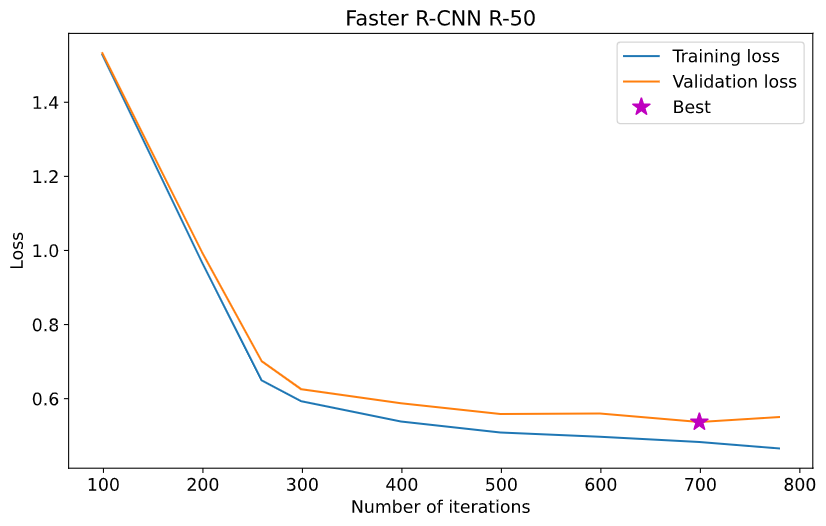
\includegraphics[width=\textwidth]{Sources/Figures/candies/Faster R-CNN R-50.png}
	\end{minipage}\hfill
	\begin{minipage}{0.5\textwidth}
		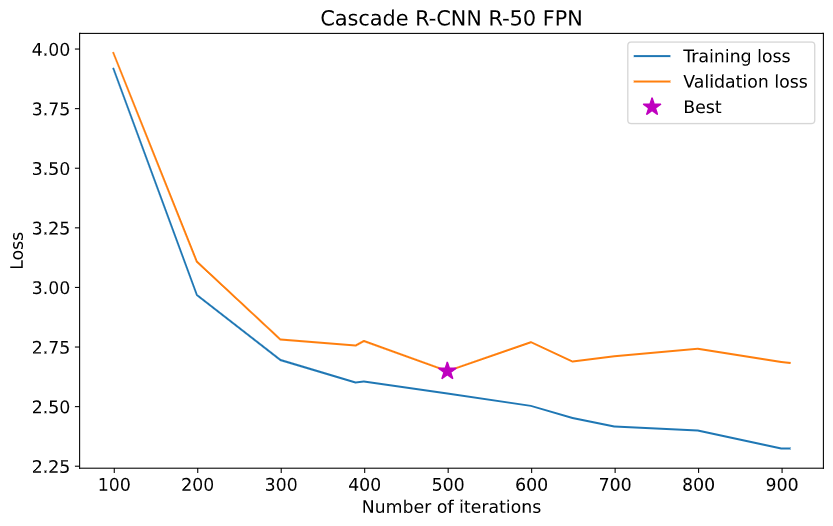
\includegraphics[width=\textwidth]{Sources/Figures/candies/Cascade R-CNN R-50 FPN.png}
	\end{minipage}\par
	\vskip\floatsep
	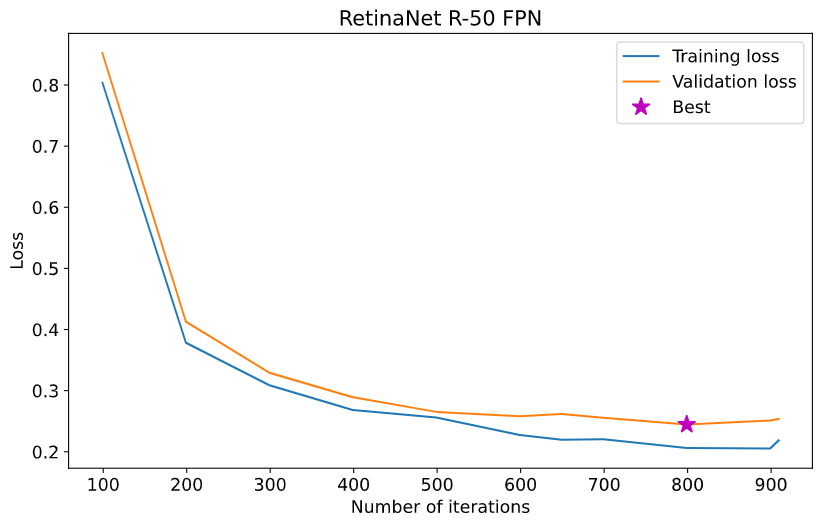
\includegraphics[width=0.5\textwidth]{Sources/Figures/candies/RetinaNet R-50 FPN.png}
	\caption{Loss curves of trained models on candies dataset.}
\end{figure}

\begin{figure}[h]
	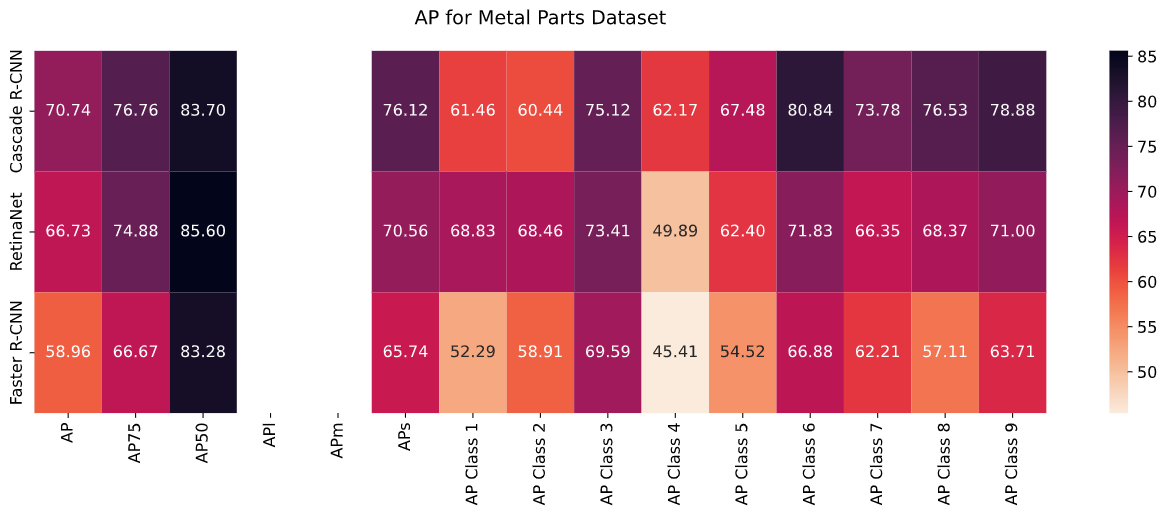
\includegraphics[width=\linewidth]{Sources/Figures/metal/metal_ap.png}
	\caption{AP table for metal parts dataset.}
\end{figure}

\begin{figure}[htp]
	\centering
	\begin{minipage}{0.5\textwidth}
		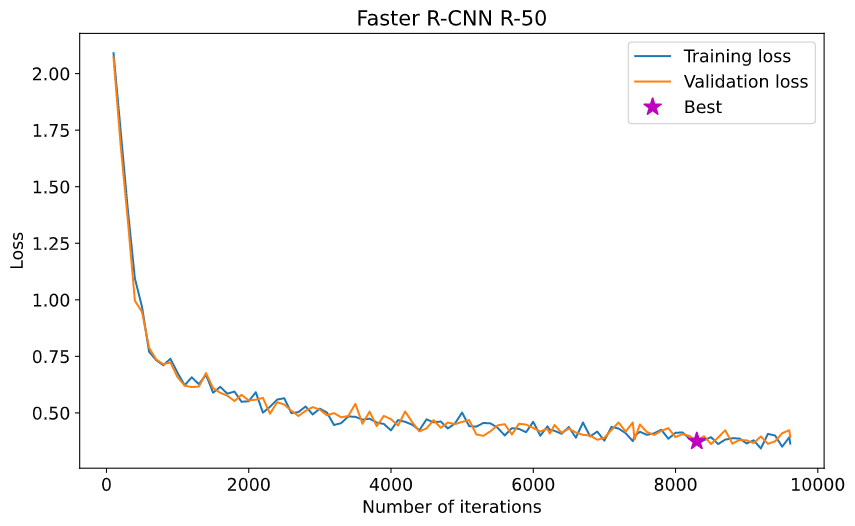
\includegraphics[width=\textwidth]{Sources/Figures/metal/metal_frcnn_loss.png}
	\end{minipage}\hfill
	\begin{minipage}{0.5\textwidth}
		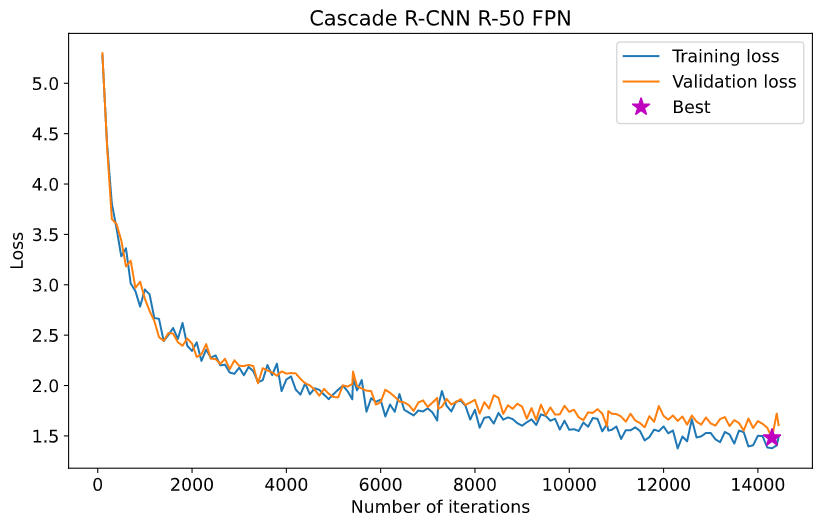
\includegraphics[width=\textwidth]{Sources/Figures/metal/metal_cascade_loss.png}
	\end{minipage}\par
	\vskip\floatsep
	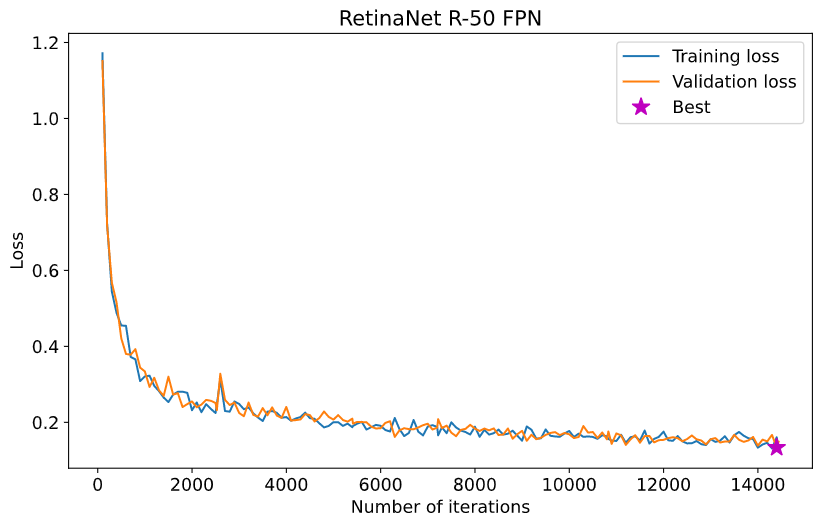
\includegraphics[width=0.5\textwidth]{Sources/Figures/metal/metal_retina_loss.png}
	\caption{Loss curves of trained models on metal parts dataset.}
\end{figure}

\begin{figure}[h]
	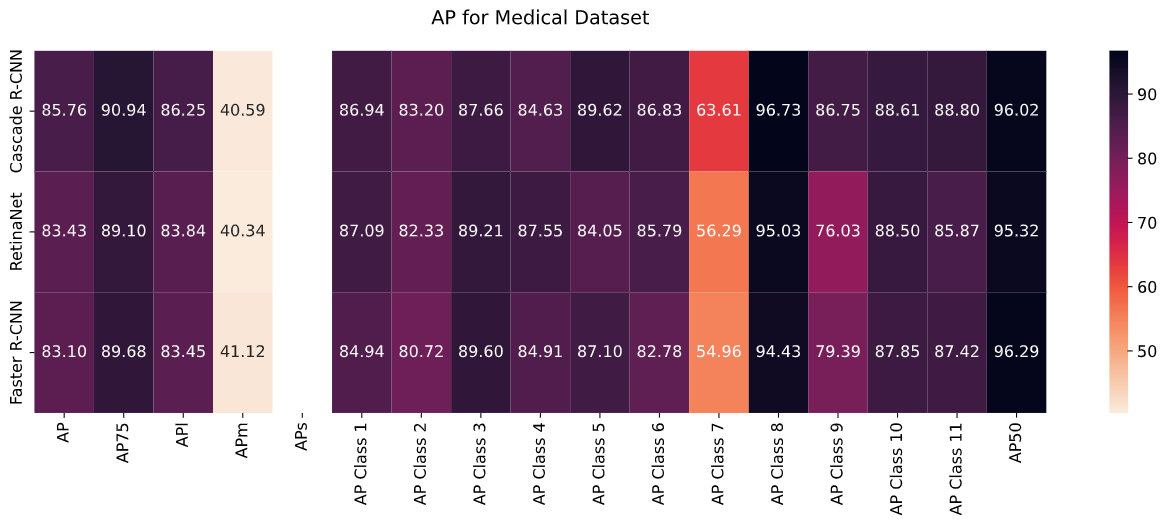
\includegraphics[width=\linewidth]{Sources/Figures/medical_ap_heatmap.png}
	\caption{AP table for medical dataset.}
\end{figure}

\begin{figure}[htp]
	\centering
	\begin{minipage}{0.5\textwidth}
		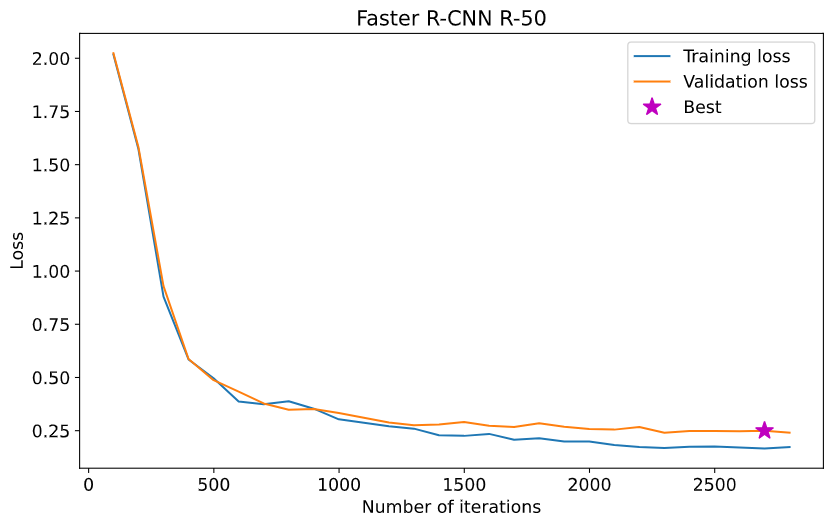
\includegraphics[width=\textwidth]{Sources/Figures/medical/frcnn_losses.png}
	\end{minipage}\hfill
	\begin{minipage}{0.5\textwidth}
		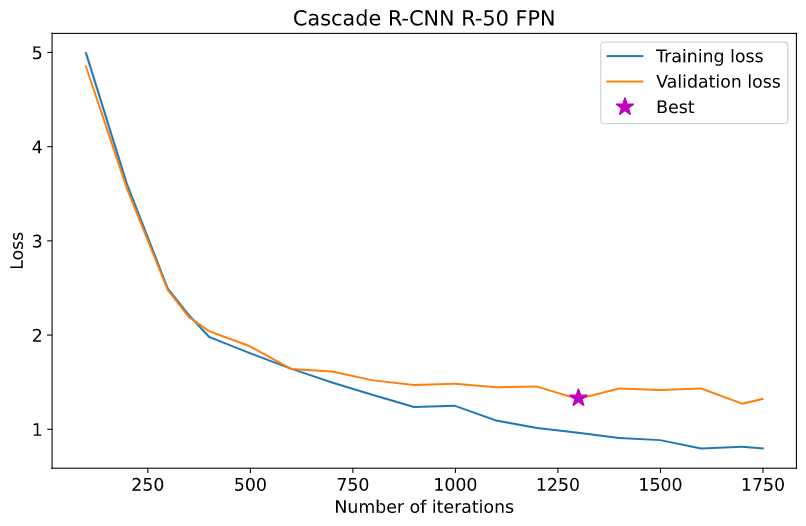
\includegraphics[width=\textwidth]{Sources/Figures/medical/cascade_losses.png}
	\end{minipage}\par
	\vskip\floatsep
	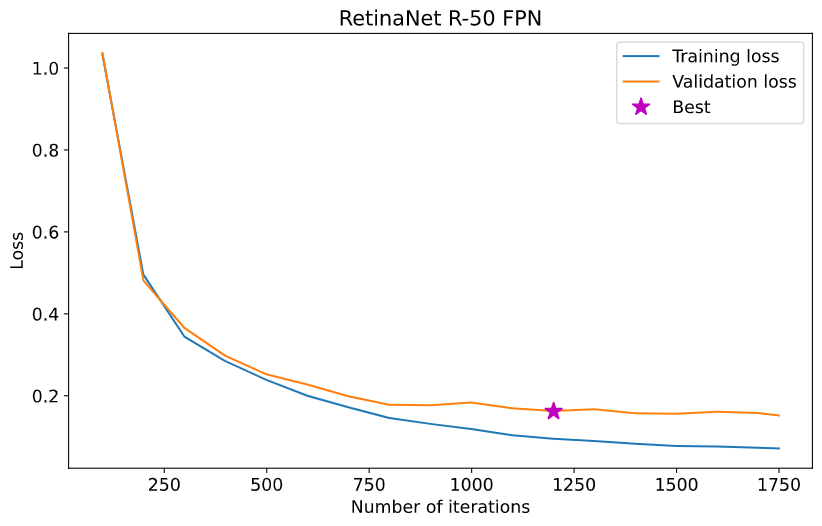
\includegraphics[width=0.5\textwidth]{Sources/Figures/medical/retina_losses.png}
	\caption{Loss curves of trained models on medical dataset.}
\end{figure}

